\chapter{Proposed Methodology}
\thispagestyle{empty}
In this chapter we will discuss about our proposed methodology and learn about every module of our system. We will find short mathematical insight of each learning algorithm used in our system. Finally overall system is summarized with an example.
\section{Proposed Text Classification System}
The key objective of our project is to design a system that can classify suspicious and non-suspicious text. \textbf{Fig} \ref{fig:proposed_model} shows an abstract view of our system.
\vspace{0.5cm}
\begin{figure}[h!]
\centering
  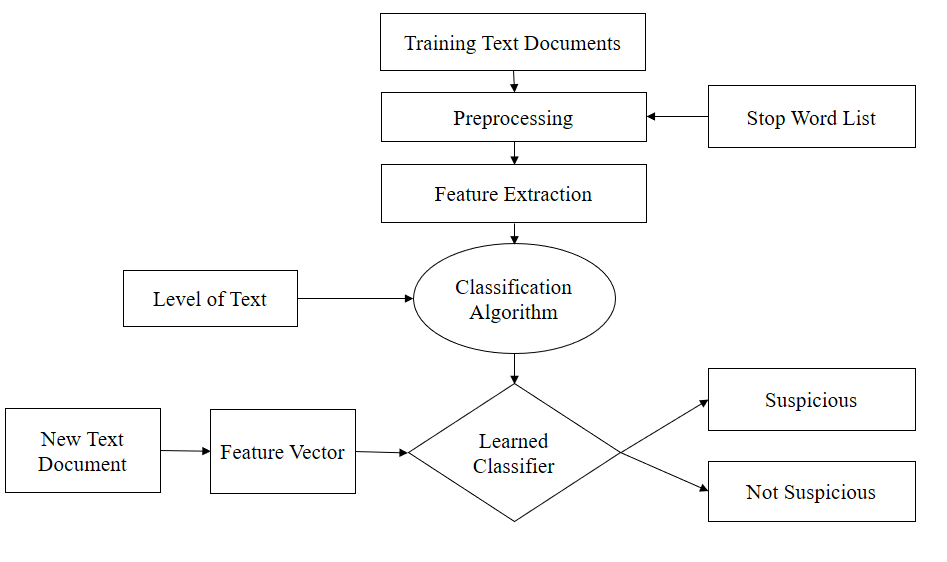
\includegraphics[scale=0.6]{Figures/proposed_model.PNG}
  \caption{Proposed Model of Suspicious Text Detection}
  \label{fig:proposed_model}
\end{figure}
 
 \section{Training Text Corpus}
 Supervised learning involves using a set of training examples that make up the training data. In linguistics, a corpus or text corpus is a large and structured set of texts nowadays usually electronically stored and processed. For a machine learning algorithm a well corpus is essential to perform according to expectation. In the corpus each training example consists of an input text and desired output value. An algorithm is then applied to the data to produce a classifier which will determine the correct output for any further valid input values. In Bengali language processing there is no corpus available which contains suspicious text. But as ours is a supervised classification system, our suspicious text detector needs a training corpus which consist of text and labels indicating whether a text is suspicious or non-suspicious. To implement this system we collect a large amount of Bangla  suspicious text. This texts are collected from online blogs, newspaper, Facebook post and other type of electronic source. Training corpus is divided into positive set (Suspicious text) and negative set (non-suspicious text). The accuracy of the learning algorithms depend on uniqueness of training examples.
 
 \section{Preprocessing}
 In natural language processing, data preprocessing is an essential step. Data preprocessing is a data mining technique that involves transforming raw data into an understandable format. Real world data is often incomplete, inconsistent, and/or lacking in certain behaviors or trends, and is likely to contain many errors. Data preprocessing is a proven method of resolving such issues. Data preprocessing is required to fill in missing values, smooth noisy data, identify or remove the outliers, and resolve inconsistencies.
 Words with no significance must be removed from the text. In our system all texts are preprocessed by the preprocessor. We use main bodies of the text to train suspicious text detector. We are going to represent our text document by list of words and their frequencies. We have a stop word list which consist of words that make no contribution to classify text. In our preprocessing section, such word will be removed by matching with stop word list. It will be very helpful to increase efficiency of the system because redundant will slow our system and increase computational complexity of the system.
 
\section{Feature Extraction}
Word frequencies will be used as feature in our proposed system. Word frequencies are used as features quite often, and although they are usually considered a basic feature, they can prove to be effective.
Terms associated with feature extraction of our system are described shortly.
\subsection{CountVectorizer}

CountVectorizers used to learn the vocabulary of a set of texts and then transform them into a data-frame that can be used for building models. CountVectorizer takes few parameter that is important for extracting feature accurately.

\subparagraph{Stop Words :}
CountVectorizer just counts the occurrences of each word in its vocabulary, extremely common words stop words will become very important features while they add little meaning to the text. In our system we do not take those words into account which improves system accuracy.
\subparagraph{Min-DF, Max-DF :}
These parameters are the minimum and maximum document frequencies words/n-grams must have to be used as features. If either of these parameters are set to integers, they will be used as bounds on the number of documents each feature must be in to be considered as a feature. If either is set to a float, that number will be interpreted as a frequency rather than a numerical limit.
\subparagraph{Max-Features :}
\texttt{max\_features} parameter is used to limit maximum number of feature used by the model. In our system we take most frequent 1000 words by using this parameter to reduce time and storage complexity.

\subsection{Word2vec}
Word2vec is used to train different learning model. Word2vec takes as its input a large corpus of text and produces a vector space, typically of several hundred dimensions, with each unique word in the corpus being assigned a corresponding vector in the space. Word vectors are positioned in the vector space such that words that share common contexts in the corpus are located in close proximity to one another in the space. Accuracy increases overall as the number of words used increases, and as the number of dimensions increases. But we should be careful about associated complexities. 

\subsection{TF-IDF}
The tf–idf is the product of two statistics, term frequency and inverse document frequency. There are various ways for determining the exact values of both statistics.

\subparagraph{Term Frequency}$tf(t,d)$, the simplest choice is to use the raw count of a term in a document, i.e., the number of times that term $t$ and occurs in document $d$.If we denote the raw count by $f_{t,d}$, then the simplest $tf$ scheme is $tf(t,d) = f_{t,d}$. Term frequencies can be calculated in  different ways,
\begin{enumerate}
    \item Term Frequency : 
    \begin{equation}
        \dfrac{f_{t,d}}{\sum_{t'\epsilon d}^{}f_{t',d}}
    \end{equation}
    \item Logarithmically scaled frequency :
    \begin{equation}
         tf(t,d)=\log(1+f_{t,d})
    \end{equation}
   
    \item To prevent bias for longer documents following equation is used:
    \begin{equation}
        tf(t,d) = 0.5 + 0.5 * \frac{f_{t,d}}{\max{(f_{t',d}\colon t'\epsilon d)}}
    \end{equation}
\end{enumerate}

\subparagraph{Inverse Document Frequency}
is a measure whether a term is common or rare across all document. IDF can be calculated by following equation,
\begin{equation}
    idf(t,d) = \log \frac{N}{\abs{1+(d\epsilon D\colon t\epsilon d)}}
\end{equation}
\noindent
%\vspace{0.5cm}
$N$ : Total number of documents in the corpus $N = \abs{D}$\newline
$(d \epsilon D\colon t\epsilon d)$ : \textrm{Number of document where term $t$ appears.}\newline
\vspace{0.5cm}
Now $tf-idf$ is calculated as,
\begin{equation}
    tfidf(t, d, D) = tf(t, d)*idf(t, D)
\end{equation}
So, Final weighting scheme of $tf-idf$ is,
\begin{equation}
        tfidf(t, d, D)=(0.5 + 0.5 * \frac{f_{t,d}}{\max{(f_{t',d}\colon t'\epsilon d)}})*\log \frac{N}{n_t}
\end{equation}
\clearpage

\section{Classification Algorithm}
After extracting feature from the text, now these features are used to train our machine learning model. Different classification algorithms have been used for training purpose.

\subsection{Intuition of Naive Bayes Classifier}
Naive Bayes is a simple technique for constructing classifiers using feature values. All naive Bayes classifiers assume that the value of a particular feature is independent of the value of any other feature, given the class variable. \textbf{Fig.} \ref{fig:NBC} shows decision boundary for Naive Bayes classifier.

\begin{figure}[h!]
    \centering
    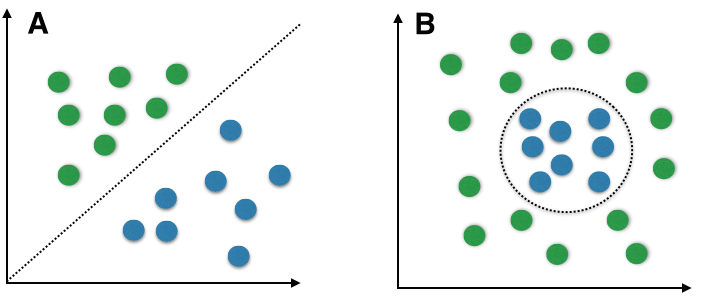
\includegraphics[scale=0.4]{Figures/naive_bayes.png}
    \caption{Naive Bayes Classifier}
    \label{fig:NBC}
\end{figure}

%%% Citation ache %%%%%%
As a popular classification algorithm, Naive Bayes algorithm [4] will be used in our system. It can be defined as Bayes theorem with a conditional independency assumption that all variables $A_{1},A_{2},...,A_{n}$ in a given category $C$ are conditionally independent with each other given $C$. 
According to Bayes rule for a text document $(T)$ and class $(C)$ we can write,
\begin{equation}
    P(C|T) = \frac{P(T|C)P(C)}{P(T)}
\end{equation}
The class we are looking for to assign this document is out of all classes the one that maximizes the probability of that class given the document.
\begin{equation}\label{eq:11}
 \begin{aligned}
     C_{MAP} & = argmax P(C|T) \\     & = argmax \frac{P(T|C)P(C)}{P(T)}\\
    & = argmax {P(T|C)P(C)}
\end{aligned}
\end{equation}
So final equation for Naive Bayes Classifier is,
\begin{equation}
     C_{MAP} = argmax P(X_{1},X_{2},...,X_{n}|C)P(C)
\end{equation}

\subsection{Intuition of Support Vector Machine}
Support vector machines are supervised learning models with associated learning algorithms that analyze data used for classification and regression analysis.  A support vector machine constructs a hyperplane or set of hyperplanes in a high- or infinite-dimensional space, which can be used for classification, regression, or other tasks like outliers detection. A good separation is achieved by the hyperplane that has the largest distance to the nearest training-data point of any class. \textbf{Fig.} \ref{fig:SVM} shows decision boundary for linear SVM.


\begin{figure}[h!]
    \centering
    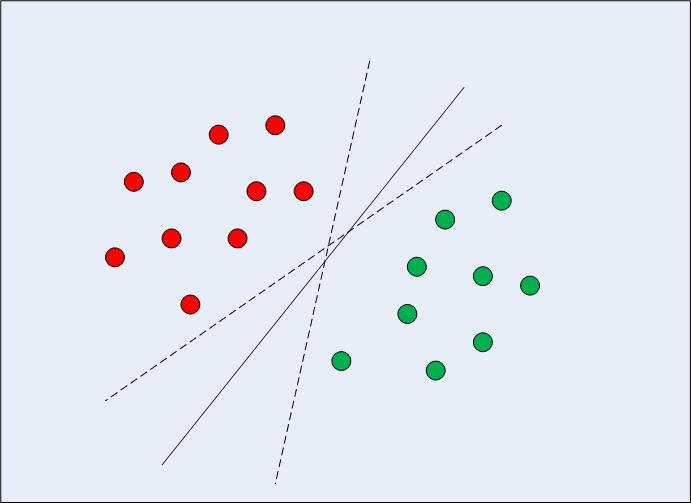
\includegraphics[scale=0.4]{Figures/svm.png}
    \caption{Support Vector Machine}
    \label{fig:SVM}
\end{figure}

SVM can perform linear classification as well as non-linear classification using kernel trick. For linear classification cost function can be written as,
\begin{equation}
    \label{cost_function_svm}
    \frac{1}{n}\sum_{i=1}^{n}\max{(0,1-y_{i}(w.x_{i}-b))} + \lambda (\lVert \mathbf{w} \rVert)^2
\end{equation}

The parameter $\lambda $ in equation 3.11 determines the trade-off between increasing the margin-size and ensuring that the samples lie on the correct side of the margin.Thus, for sufficiently small values of $\lambda $, the second term in the loss function will become negligible, hence, it will behave similar to the hard-margin SVM, if the input data are linearly classifiable, but will still learn if a classification rule is viable or not.
\par\noindent
For non-linear classification with SVM kernel trick is used. Some common kernel tricks used in machine learning are,
\begin{itemize}
    \item Gaussian radial basis function:
    \begin{equation}
         k(x_{i}, x_{j}) = \exp{(-\gamma(\lVert \mathbf{x_{i}-x_{j}} \rVert)^2)}
    \end{equation}
    \item Polynomial Kernel (homogeneous):
    \begin{equation}
        k(x_{i}, x_{j}) = (x_{i}\cdot x_{j})^d
    \end{equation}
     \item Polynomial Kernel (inhomogeneous):
     \begin{equation}
         k(x_{i}, x_{j}) = (x_{i}\cdot x_{j}+1)^d
     \end{equation}
    \item Hyperbolic tangent:
    \begin{equation}
       k(x_{i}, x_{j}) = tanh(kx_{i}\cdot x_{j}+c) 
    \end{equation}
\end{itemize}
Above equations expresses the kernel trick which are really important for classification and regression analysis.

\subsection{Intuition of Logistic Regression}
Logistic Regression is a binary classification model that predicts a binary outcome based on some features. The output of logistic regression depends on logistic function. The logistic function is a sigmoid function, which takes any real input and outputs a value between zero and one. For binary logistic regression selecting the threshold value is an important task, everything below threshold will considered as $0$ or negative otherwise it will be $1$ or  positive.\textbf{Fig.} \ref{fig:logistic_regression} shows decision boundary for logistic regression.  

\begin{figure}[h!]
    \centering
    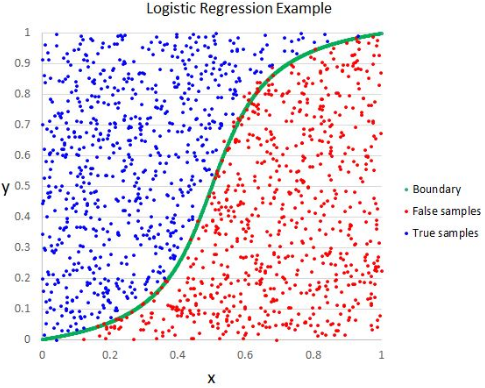
\includegraphics[scale=0.7]{Figures/logistic_regression.png}
    \caption{Logistic Regression}
    \label{fig:logistic_regression}
\end{figure}
For Logistic Regression the definition of logistic function or hypothesis function is,
\begin{equation}
    h_{\theta}(x) =  \frac{1}{1+\exp({-\theta^T x})}
\end{equation}
we can not use the cost function of Linear regression because if we that cost function the decision boundary will be non convex. Now cost function for Logistic regression is,
\begin{equation}
    J(\theta) = \frac{1}{m}\sum_{i-1}^{m}cost(h_{\theta}(x^{i}),y^{i})   
\end{equation}

\[
cost(h_{\theta}(x), y) = 
\begin{cases}
    -\log (h_{\theta}(x)) & \texttt{if } y = 1\\
     -\log (1-h_{\theta}(x)) & \texttt{if } y = 0
\end{cases}
\]
\par
\noindent
Here,\\
$m = $ Number of training examples.\\
$h_{\theta}(x^{i}) = $ Hypothesis function of $i_{th}$ training example\\
$y^i = $ Input label of $i_{th}$ training example.\par
\vspace{0.5cm}
\noindent
Writing cost function in this way guarantees that cost function $J(\theta)$ is convex for logistic regression.
.
\subsection{Intuition of K-Nearest Neighbor}
The k-nearest neighbors algorithm (k-NN) is a non-parametric method used for classification and regression. In both cases, the input consists of the k closest training examples in the feature space. In k-NN classification, the output is a class membership. An object is classified by a majority vote of its neighbors, with the object being assigned to the class most common among its k nearest neighbors. (k is a positive integer, typically small). If k = 1, then the object is simply assigned to the class of that single nearest neighbor.
\begin{figure}[h!]
    \centering
    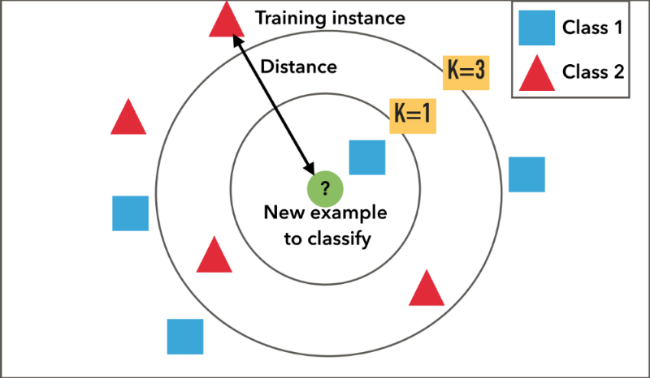
\includegraphics[scale=0.35]{Figures/knn.png}
    \caption{K-Nearest Neighbor}
    \label{fig:knn}
\end{figure}
\par
\noindent
\textbf{Fig.} \ref{fig:knn} represents K-NN decision boundary. K nearest neighbors is a simple algorithm that stores all available cases and classifies new cases based on a similarity measure (e.g., distance functions). Most commonly used three different distance function of K-NN are,

\begin{enumerate}
    \item Euclidean distance function :
    \begin{equation}
        \sqrt{\sum_{i=1}^{k}(x_i-y_i)^2}
    \end{equation}
    \item Manhattan distance function :
    \begin{equation}
         \sum_{i=1}^{k}\abs{(x_i-y_i)}
    \end{equation}
    \item Minkowski distance function :
    \begin{equation}
        ({\sum_{i=1}^{k}(\abs{x_i-y_i})^q)})^\frac{1}{q}
    \end{equation}
    
\end{enumerate}
\par\noindent
All three distance measures are only valid for continuous variables. In the instance of categorical variables the Hamming distance must be used. It also brings up the issue of standardization of the numerical variables between 0 and 1 when there is a mixture of numerical and categorical variables in the dataset. Hamming distance for k-nearest neighbor can be calculated as follows,
\begin{equation}
    D_H = \sum_{i=1}^{k}\abs{(x_i-y_i)}
\end{equation}
$$ D = 0 \texttt{ if } x = y $$
$$ D = 1 \texttt{ if } x\neq y $$
\par\noindent
Choosing the optimal value for K is best done by first inspecting the data. In general, a large K value is more precise as it reduces the overall noise but there is no guarantee.  Cross-validation is another way to retrospectively determine a good K value by using an independent dataset to validate the K value. Historically, the optimal K for most datasets has been between 3-10. That produces much better results than 1NN.
\clearpage

\subsection{Intuition of Decision Tree}
Decision tree learning is a method commonly used in machine learning. In a Decision tree each interior node  corresponds to one of the input variables; there are edges to children for each of the possible values of that input variable. Each leaf represents a value of the target variable given the values of the input variables represented by the path from the root to the leaf. \textbf{Fig.} \ref{fig:DCT} shows a simple decision tree used for classification.
\begin{figure}[h!]
    \centering
    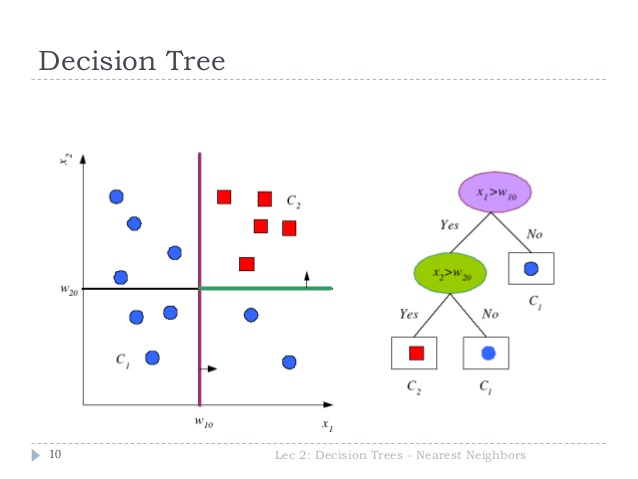
\includegraphics[scale=0.4]{Figures/decision_tree.jpg}
    \caption{Decision Tree}
    \label{fig:DCT}
\end{figure}

A decision tree is built top-down from a root node and involves partitioning the data into subsets that contain instances with similar values. Entropy is used to calculate the homogeneity of a sample. To build a decision tree, we need to calculate two types of entropy using as follows,
\begin{enumerate}
    \item Entropy using one attribute :
    \begin{equation}
         E(S) = \sum_{i=1}^{c}-P_i \log_2P_i
    \end{equation}
    \item Entropy using two attributes :
    \begin{equation}
        E(S) = \sum_{c\epsilon X}{}P(C)E(C) 
    \end{equation}
    
\end{enumerate}
\par\noindent
In this section, we gain simple intuition about some classification algorithm that will be used in our model. 


\section{Text Classification Example}
Our whole system is divided into two phases, one is training phase and another is testing phase.
\subsection{Training Phase}
\textbf{Fig.} \ref{fig:TP} summarizes our whole training process. A sample text is processed by using tokenization process. Then feature is extracted from the text and used to learn our classifier model.
\vspace{1cm}
\begin{figure}[h!]
    \centering
    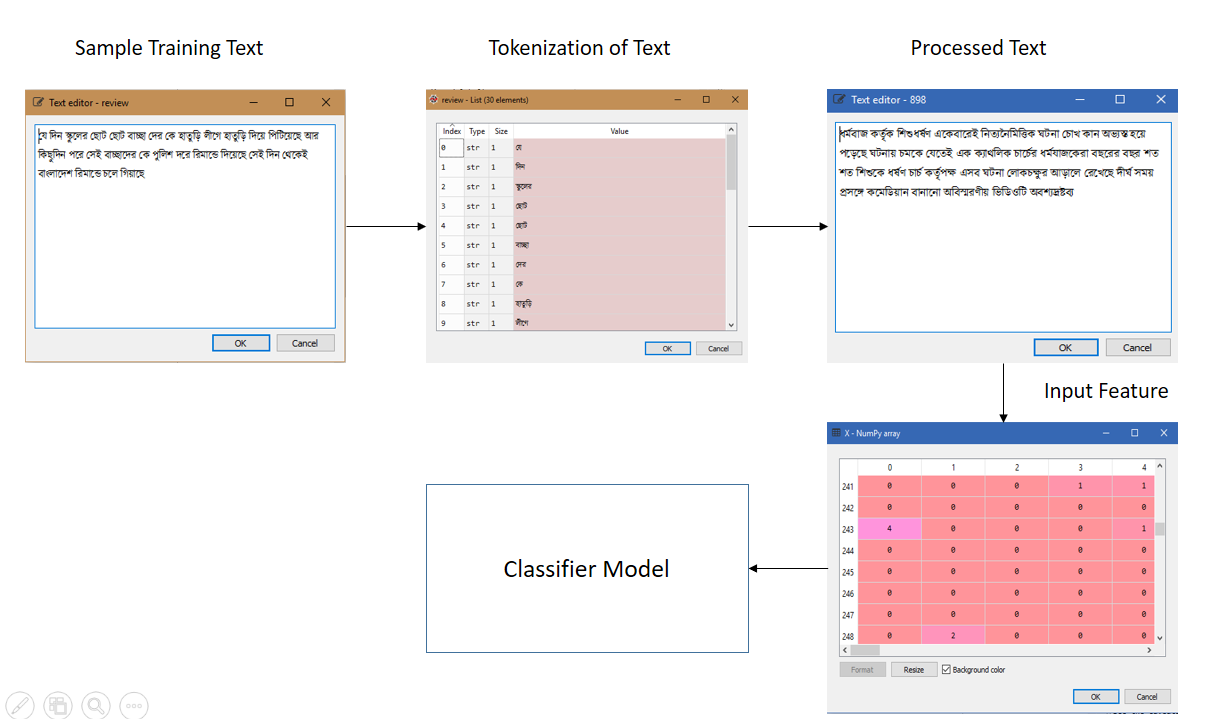
\includegraphics[width=15cm,height=14cm]{Figures/training_phase.PNG}
    \caption{Training Process}
    \label{fig:TP}
\end{figure}
\clearpage
\subsection{Testing Phase}
Whole testing process can be summarized by \textbf{Fig.} \ref{fig:TEP}. Sample texts are taken to test the system. After processing using feature extraction method feature is extracted and this features are used to classify text as suspicious and non-suspicious.

\begin{figure}[h!]
    \centering
    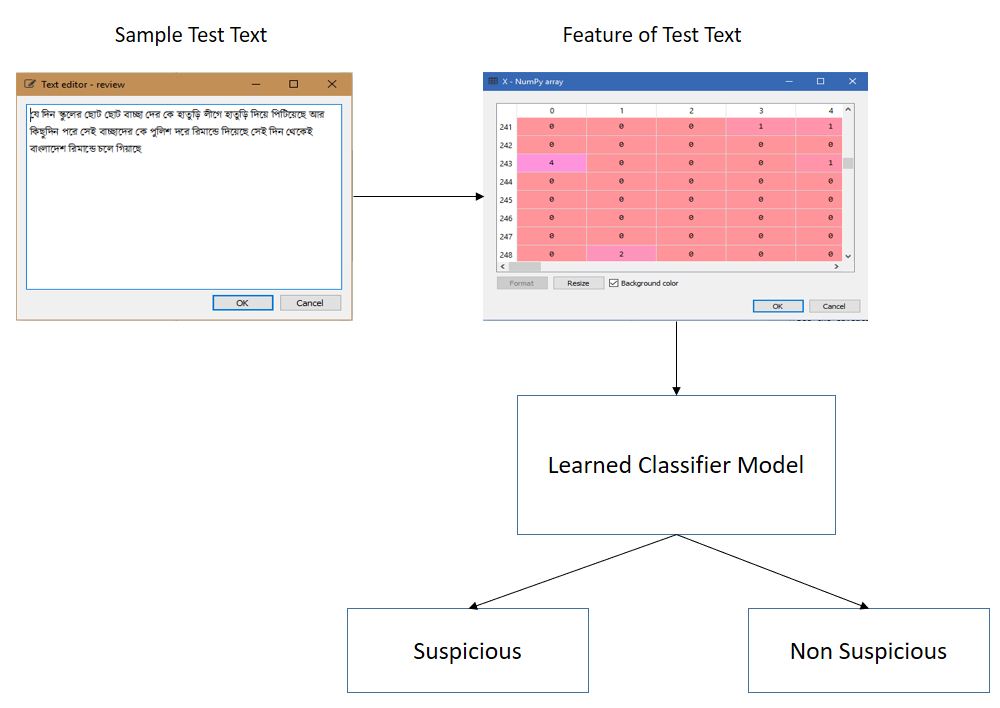
\includegraphics[width=15cm,height=14cm]{Figures/testing_phase.PNG}
    \caption{Testing Process}
    \label{fig:TEP}
\end{figure}
